\chapter{Background}
\section{SPARK}
SPARK\footnote{Short for SPADE Ada Kernel} is a formally-defined high-level
programming language designed for writing high integrity systems. It is based on
Ada, which is itself a statically typed programming language with a strong focus
on security and safety.

The SPARK language is a subset of Ada with additional features inserted as
annotations by means of Ada comments. Since compilers ignore comments and SPARK
is a true subset of Ada, any correct SPARK program is a correct Ada programm and
can be compiled using existing Ada compilers, such as GNAT, which is part of the
GNU compiler collection (GCC) \cite{gcc}. However, since annotations are an
integral part of SPARK, it would be misleading to simply consider SPARK a
constrained version of Ada. SPARK should be viewed as a programming language in
its own right. The following list summarizes the Ada restrictions imposed by
SPARK:

\begin{itemize}
	\item No access types (pointers)
	\item No recursion
	\item No exceptions
	\item No goto
	\item No anonymous and aliased types
	\item No functions with side-effects
	\item No dynamic array bounds
	\item No dynamic memory allocation
	\item No dynamic dispatching
\end{itemize}

The annotations are processed by SPARK tools. These tools perform static
analysis of the source code. The annotations allow the tools to do data and
information flow analysis as well as proof the absence of runtime errors. This
means that SPARK tools allow to formally verify, that a given program is free
of errors such as division by zero, out-of-bounds array access etc. The
following types of errors that can be proven to be absent using SPARK:

\begin{itemize}
	\item Incorrect indexing of arrays
	\item Overflows
	\item Division by zero
	\item Type range violations
	\item Memory exhaustion
	\item Dangling pointers
\end{itemize}

On top of these properties, the usage of pre-/post-conditions and assertions
allow to prove additional functional properties. A proof of (partial
\footnote{Termination cannot be shown}) correctness of SPARK programs is
achievable. This allows to formally show the correspondence of an implementation
with a formal specification.

It is also interesting to note, that SPARK has support for tasking in the form a
profile called RavenSPARK \cite{RavenSPARK}.

SPARK is a mature technology and has garnered quite some interest since it has
been used successfully in several industrial projects TODO:ref. It is primarily
employed in the field of avionics, space, medical systems and in the defense
industry.

\subsection{Design rationale}
The main driving factors behind the design of SPARK are shortly described here:

\begin{description}
	\item[Logical soundness] \hfill \\
		The language must not contain any ambiguities and defined specified.
	\item[Complexity of formal language definition] \hfill \\
		The language must be simple to specify formally.
	\item[Expressive power] \hfill \\
		The language must have rich enough to implement real systems.
	\item[Security] \hfill \\
		All language rules must be statically checkable with reasonable effort
		(within polynomial time).
	\item[Verifiability] \hfill \\
		Program verification must be tractable for industrial scale projects.
	\item[Bounded space and time requirements] \hfill \\
		Resource requirements must be determined statically.
\end{description}

\subsection{Example}
The following listing illustrates how annotations are used to specify the
contract of a subprogram.

\begin{lstlisting}[language=Ada]
type Color_Type is (Red, Green, Blue);

procedure Exchange (X, Y: in out Color_Type);
--# derives X from Y &
--#         Y from X;
--# post X = Y~ and Y = X~;
\end{lstlisting}

The declaration of the \texttt{Exchange} procedure states that it has two
parameters \texttt{X} and \texttt{Y} which are of mode \texttt{in out}. This
means that the values of both parameters are imported (\texttt{in}) and exported
(\texttt{out}).

Since the specification does not contain a \texttt{global} annotation, no other
state (e.g. global variables) is accessed. The \texttt{derives} annotations
state the data flow: the value of X is derived from Y and vice versa.

Lastly, the postconditions specify what the values of X and Y are after the
procedure has been executed. An identifier decorated with the tilde symbol
($\sim$) indicates the initial imported value of the variable. Thus the post
annotation states, that X will be assigned the initial value of Y and likewise
for Y.

It should be noted, that the \texttt{Color\_Type} is a \emph{distinct}
enumeration type which \emph{cannot} be mixed with other types.

An in-depth discussion of the SPARK programming language can be found in
\cite{BarnesSPARK}.

\subsection{SPARK 2014}
At the time of writing\footnote{June 2013} the SPARK language is undergoing a
major transformation. The goal is to extend the subset of Ada included in SPARK,
and to make use the new Ada 2012 specification features \cite{Ada2012}. The use
Ada aspects will be used instead of the annotations in the form of special
comments. It is expected to be released in 2014 \cite{SPARK2014:Announcement}.

Since the development of SPARK 2014 is currently ongoing, the kernel is
implemented using the existing SPARK 2005 language and tools.

\section{Intel x86 Architecture}
\section{Virtualization}
Virtualization is an established architectural concept in computer science and
has been in use since decades. Operating systems for example provide virtual
address spaces to application processes, giving them the illusion of unlimited,
continuous memory. An application does not need to take care of complex memory
management tasks and the operating system is able to optimize the usage of
physical memory. Another common example is the virtualization of devices such as
virtual CD-ROM drives directly using a file-based backend for data I/O.

Hardware or platform virtualization is the process of creating virtual computer
hardware that acts like real hardware. The virtualization is performed on the
host machine by special software, called a hypervisor\index{hypervisor} or
virtual machine monitor (VMM\index{VMM}). These two terms are synonyms, for
consistency we will use VMM throughout this document. VMMs are classified into
two types see figure \ref{fig:vm-classification}.

\begin{figure}
	\centering
	\begin{subfigure}[b]{0.24\textwidth}
		\centering
		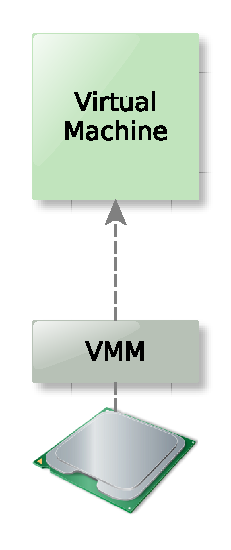
\includegraphics[width=\textwidth]{images/type-1-vmm}
		\caption{\emph{Type I, native or bare metal VMM.} Runs directly on the
		hardware in the most privileged processor mode.}
	\end{subfigure}
	\qquad
	\begin{subfigure}[b]{0.24\textwidth}
		\centering
		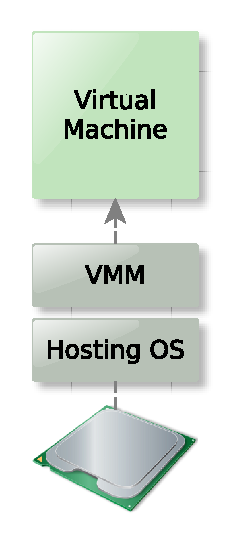
\includegraphics[width=\textwidth]{images/type-2-vmm}
		\caption{\emph{Type II or hosted VMM.} The VMM runs on top of a
		conventional operating system and uses OS services.}
	\end{subfigure}
	\caption{VMM classification}
	\label{fig:vm-classification}
\end{figure}

Software that runs in a virtualized environment is called guest software. The
words host and guest are used to distinguish the software that runs on the
physical machine from the software that runs on the virtual machine
\cite{wiki:virtualization}.

By using virtualization and scheduling techniques, a VMM multiplexes the real
hardware of a computer making it possible to run multiple guests in
parallel\footnote{On multicore machines in parallel, on single-core machines
pseudo-parallel} on one machine. This is the most common use-case for
virtualization: The consolidation of operating system instances on one server to
save power and to improve hardware-resource utilization.

A guest program is separated from the real hardware of a machine, direct access
is restricted and can be controlled by the host VMM. Since the VMM has complete
control over the hardware of a system and all guest software, virtualization is
also useful for separation purposes. The VMM can allow certain communication
channels between guest software while restricting others. One guest could have
access to the network card, while others share a page in memory but have no
access to hardware devices.

The principle idea of virtualization is to run guest code in the virtual machine
and intercept privileged operations which access critical resources or system
properties. A guest traps into the VMM if such an instruction is executed and
the VMM acts according to the situation. This method is used to implement a
technique called "trap and emulate". For example if a guest accesses a device
which is emulated by the VMM, access to the virtual device causes a trap into
the VMM. The VMM itself or a special monitor VM then emulates the requested
operations of the guest software by directly modifying the state of the virtual
processor or memory of the guest VM.

A trap from the guest into the VMM is a costly operation. To reduce traps,
mechanisms in modern processors have been introduced to support the VMM in
creating a virtual machine environment. Processor features like Intel VT-x, EPT
and VT-d not only improve the performance of a virtual machine by avoiding traps
but also allow the VMM software code to be much simpler.

\section{Separation Kernel}
In a system with high requirements on security, functions relevant
to guarantee these requirements must be isolated from the rest of
the system and consolidated in a Trusted Computing Base (TCB)\index{TCB}.
To be trusted, this code must be as minimal as possible to allow formal
verification of code correctness. Lampson et al.
\cite{Lampson:1991:ADS:121133.121160} define the TCB of a computer system as:
\begin{quote}
	A small amount of software and hardware that security depends on and
	that we distinguish from a much larger amount that can misbehave without
	affecting security.
\end{quote}

A separation kernel\index{kernel} (SK\index{SK}) is therefore the fundamental
part of the TCB as its main purpose is to enforce the separation of all other
components making such a component-based system possible in the first place. The
concept of separation kernels was introduced by John Rushby in a paper from 1981
\cite{rushby1981}. While the original paper describes a distributed system, it
is more illustrative to think of it as multiple components which behave as if
they were running on dedicated hardware. The separation kernel must guarantee
that the components can only interact according to a well-defined policy while
running on the same physical hardware.

A system policy dictates the partitioning of hardware resources like CPU, memory
or devices to components. The kernel guarantees this isolation by emulating a
suitable runtime environment for each component, creating the impression of
multipe (virtual) machines. By using modern virtualization techniques, the
kernel is able to delegate certain management tasks to the hardware. This allows
the separation kernel code to be relatively simple, which is a precondition for
formal verification of software.

Because of the simplicity requirement, a system running on top of a separation
kernel is relatively static. The system policy is compiled to a suitable format
on system integration and can not change during runtime. This is is also the
main difference between the separation kernel concept and microkernels which
provide hardware abstraction layers and advanced mechanisms for inter-process
communication (IPC\index{IPC}). A separation kernel does not implement such
functionality, it's sole purpose is to guarantee component separation according
to policy. Policy-writers must make sure that the system specification is sound
and that only allowed communication channels are specified between components.
Of course, this task can be simplified by providing support tools.

\subsection{Subjects}
The separation kernel isolates parts of the TCB into multiple
components\index{component} interacting over well-defined interfaces. In this
paper, such components are called subjects\index{subject}.

As said, only the absolutely necessary features to guarantee subject separation
are present in a separation kernel. Advanced features required to isolate a
complex subject are implemented as dedicated non-privileged subjects. A complex
subject could be a complete operating system like Linux\index{Linux}.

To allow more flexibility, a separation kernel could also use a dedicated
subject to offload management and policy decision tasks. Such a subject runs in
normal unprivileged mode but is allowed to interact with the kernel over a
specialized interface.

\section{Motivation}
As outlined in the previous section, software must be simple to establish trust
in the correct functioning of the code either through manual review or formal
verification. Even though the tools to perform formal verification
automatically are progressing fast, the constraints on the software to be
verified are still severe. If the SLOC\footnote{Source lines of
code}\index{SLOC} count of a software project exceeds a critical threshold, it
is no longer possible to automatically proof integrity and security
requirements or to perform a manual review, the code base is just too large.

This is the reason why common operating system kernels are not suitable to be
used as a foundation to create a high assurance system with a small TCB. The
Linux\index{Linux} kernel currently has a SLOC count of over 14 million lines
of code. While functionality can be loaded as modules, Linux is still a
monolithic kernel at the architectural level with the complete code running in
the same address space and privilege level. A crash or programming error in a
device driver for example can be used to exploit the complete system.

While commercial separation kernel products exist on the market, there is
currently no open-source SK\index{SK} available. This is a major drawback for
implementers of a high assurance system since they must trust the most
fundamental building block, the kernel, without the possibility to review the
code or the verification documents (if any). It is of course also impossible to
adapt the kernel code to the specific needs of a customer, which may hinder
development of the final system.

The goal of this project is to provide a freely-available SK with a permissive
licensing\index{license} model allowing to review and modify the source code.
It should also be possible to re-apply all tools making the proofs
reproducible. In the eyes of the authors, only this approach is viable in
environments where high integrity and security is demanded.

There have been many advances in hardware support for virtualization, allowing
the design of a much simpler kernel than without those features. The authors
believe that now is a good time to start a separation kernel project which
benefits from these latest advances.

\section{Goals}
The main goal of this project is to implement a freely-available, open-source
separation kernel. The kernel sources will be licensed under the GNU General
Public License (GPL\index{GPL}, REF).

SPARK is used as main implementation language as this guarantees the
availability of advanced and approved tools to write code for high assurance
environments. The SPARK tools will be used to show certain properties of the
kernel code, especially proof of absence of runtime errors is desired.

The code of the kernel must be minimal to have a small TCB.

Non-timing critical operations should be implemented in a special trusted
subject written in SPARK. This subject is called $\tau$0 and is considered an
integral part of the kernel. TODO: explain time-critical and real-time in this
context. While keeping the main kernel as simple as possible, this allows for
later adoption of more dynamic mechanisms for resource handling and scheduling.

The target platform of the SK is 64-bit Intel. No abstraction layer will be
provided to support other processor architectures. Such a layer, if ever needed,
could be added later. Instead, the kernel should leverage the latest hardware
features of the Intel platform.

The main task of the SK is to separate subjects. This is why it must only allow
intended data flows according to the policy and it should prevent or limit
possible side- or covert-channels.

\section{Related work}
This section presents similar and related projects. While they share many
similarities with the Muen kernel, the main difference is ...TODO

\subsection{seL4}
seL4 is microkernel of the L4 \cite{Liedtke:1996:TRM:234215.234473} family which
has been formally verified. It aims to provide high assurance of functional
correctness by means of machine-checked formal proofs. Using the theorem prover
Isabelle/HOL \cite{Nipkow-Paulson-Wenzel:2002}, it has been shown that the C
implementation correctly implements an abstract specification.

To our knowledge seL4 is the most advanced project in the field of formal
verification combined with operating system research. Unfortunately its
availability and use is rather limited by restrictive licensing. While parts of
the seL4 project are available for non-commercial use, the source code of the
kernel has not been published. Thus it is not possible to reproduce the formal
proof.

\subsection{XtratuM}
XtratuM is a type 1 hypervisor specially designed for real-time embedded
systems. It is developed by the Real-Time Systems group of the Universidad
Politécnica de Valencia. It uses para-virtualization to provide one or more
virtual execution environments for so called partitions. This means software
running as partitions must be modified accordingly to run on top of XtratuM.

The processor privilege mechanism (supervisor and user mode) is used to
separate the hypervisor from partitions.

The whole project is open-source and published under the GPL license. It is
implemented in C and assembly. While it supports various platforms such as
LEON2/3 (PowerPC) and Intel x86, it does not support Intel x86-64.

\subsection{NOVA}
NOVA is a recursive acronym and stands for NOVA OS Virtualization Architecture
\cite{Steinberg:2010:NMS:1755913.1755935}. It applies microkernel construction
principles to create a virtualization environment. Its authors have coined
the term microhypervisor\index{microhypervisor} which is short for
microkernelized hypervisor.

NOVA has been developed from scratch with the goal to achieve a thin hypervisor
layer, a users-level virtual-machine monitor (VMM) and additional unprivileged
components to reduce the attack surface on the most privileged code and thus
increase the overall system security. It runs on Intel and AMD x86 processors
with support for hardware virtualization and is implemented in the C++
programming language. The source code is publicly available TODO:Ref and has
been released under the GPL open-source license.

While NOVA is a very promising architecture it has some drawbacks: the choice of
programming language (C++) and its dynamic nature, in general a very desirable
property, increases the verification complexity to the point where it might be
unfeasible.

\subsection{Commercial separation kernels}
There are several commercial offerings for separation kernels by various
vendors:

\begin{itemize}
	\item INTEGRITY-178B by Green Hills Software, Inc. is a separation kernel
		certified against the separation kernel protection profile (SKPP).
	\item PikeOS by SYSGO AG is a microkernel based real-time OS.
	\item LynxSecure by LynuxWorks Inc. is a type 1 embedded hypervisor for the
		Intel x86 architecture.
	\item VxWorks MILS Platform by WindRiver Inc. is a type 1 hypervisor–based,
		SKPP-conformant MILS separation kernel–based platform.
\end{itemize}

None of these companies publish detailed technical documentation or provide
access to source code. Thus there is not enough information available for a
thorough technical analysis to asses the assurance provided by these kernels
(e.g. if the kernels are suitable for formal verification and what kind of
verification has been performed).
